\documentclass[12pt,a4paper]{report}
\usepackage[a4paper,
    left=1.25in,
    right=1in,
    top=1in,
    bottom=1in]{geometry} % Required for inserting images
\usepackage{fullpage}
\usepackage{titletoc}
\usepackage[titles]{tocloft}
\usepackage{newtxtext}
\usepackage{newtxmath}
\usepackage{setspace}
\onehalfspacing

\usepackage{lipsum}
\usepackage{acronym}
\usepackage{graphicx}
\graphicspath{ {./images/} }

\renewcommand*\contentsname{Table of Contents}

% Redefine the \numberline command for figures
\newlength{\mylen}
\renewcommand{\cftdotsep}{0.5}
\renewcommand{\cftfigpresnum}{\hspace*{-1.5em}\figurename\enspace}
\renewcommand{\cftfigaftersnum}{:}
\settowidth{\mylen}{\cftfigpresnum\cftfigaftersnum}
\addtolength{\cftfignumwidth}{\mylen}


\renewcommand{\cftdotsep}{0.5}
\renewcommand{\cfttabpresnum}{\hspace*{-1.5em}\tablename\enspace}
\renewcommand{\cfttabaftersnum}{:}
\settowidth{\mylen}{\cfttabpresnum\cfttabaftersnum}
\addtolength{\cfttabnumwidth}{\mylen}


\titlecontents{chapter}
[5.5em] %5.3
{\smallskip}
{\contentslabel[\bfseries{\chaptername}~\thecontentslabel{:}]{5.5em}\textbf}%\thecontentslabel
{\hspace*{-5.5em}\textbf}% unnumbered chapters
{\titlerule*[0.35pc]{.}\contentspage}[\smallskip]%

\titlecontents{section}
[1.5em] % i
{\smallskip}
{\thecontentslabel\enspace}%\thecontentslabel
{\hspace*{-5.5em}}
{\titlerule*[0.35pc]{.}\contentspage}%]

\titlecontents{subsection}
[7.12em] %
{\smallskip}
{\thecontentslabel\enspace}%\thecontentslabel
{\hspace*{7.12em}}
{\titlerule*[0.35pc]{.}\contentspage}

\makeatletter
\renewcommand{\@makechapterhead}[1]{%\vspace*{50 pt}%
{\setlength{\parindent}{0pt}\normalfont\centering
\bfseries\fontsize{14pt}{16pt}\selectfont\MakeUppercase{\chaptername~\thechapter: #1}
\par\nobreak\vspace{16 pt}}}
\makeatother

\makeatletter
\renewcommand{\@makeschapterhead}[1]{%\vspace*{50 pt}%
{\setlength{\parindent}{0pt}\normalfont\centering
\bfseries\fontsize{14pt}{16pt}\selectfont\MakeUppercase{#1}
\par\nobreak\vspace{16 pt}}}
\makeatother

\title{Major}
\author{Swetraj Paudel}
\date{May 2024}

\setlength{\parindent}{0pt}

\begin{document}
\begin{titlepage}
    \thispagestyle{empty}
    \begin{center}
    
    \vspace*{\fill} % * makes latex to not ignore the command
    {\large \textbf{TRIBHUVAN UNIVERSITY
}\par}
{\large \textbf{INSTITUTE OF ENGINEERING
}\par}
\vspace{8pt}
PURWANCHAL CAMPUS \par
DHARAN, SUNSARI
\vspace{24pt}


\includegraphics[scale=0.45]{tu}
\vspace{14pt}

{Major Project Proposal/Report on\par}
\vspace{7pt}
{
    \textbf{Design, Modeling, and Kinematic-Dynamic Analysis of} 
    \par
    \textbf{a Stick Counting and Packaging System}
\par
}

\vspace{14pt}
{BY\par} 
\vspace{7pt}
    
{SEWAK SUNAR - PUR080BME051\par}
{PRIT NARAYAN YADAV - PUR080BME063\par}
{INDRA NARAYAN SHA - PUR080BME062\par}
{SASHI MANDAL - PUR080BME049\par}

\vspace{14pt}
{TO\par}
\vspace{7pt}
{DEPARTMENT OF MECHANICAL ENGINEERING \par}
% {SUNSARI, NEPAL \par}
{11th June, 2026 \par}
    \vspace*{\fill}

    \end{center}
\end{titlepage}



\pagenumbering{roman}

\chapter*{Acknowledgement}
\addcontentsline{toc}{chapter}{Acknowledgement}
\label{acknowledgement}
\lipsum[2-4]
I am was privellage to work under Prof. Anu Sh

\chapter*{Abstract}
\addcontentsline{toc}{chapter}{Abstract}
\label{abstract}
Mechanical automation plays a vital role in improving the efficiency and reliability of repetitive industrial operations. This project focuses on the **design, modeling, and kinematic-dynamic analysis of a semi-automatic stick counting and packaging mechanism**. The primary objective is to study and evaluate the performance of various mechanical mechanisms that can be integrated to achieve accurate stick counting, bundle formation, and packaging operations.

\vspace{12px}
The proposed system consists of a stick feeding mechanism, a purely mechanical counting mechanism, an intermittent motion transfer mechanism, and a bundle holding and packaging mechanism. The study emphasizes the application of machine design principles, including linkages, ratchet-pawl systems, cam mechanisms, and intermittent motion mechanisms, to achieve synchronized and repeatable operations without relying on complex electronic control systems.

\vspace{12px}
The project methodology involves conceptual design, engineering calculations, three-dimensional modeling using FreeCAD, and kinematic and dynamic analysis to investigate the motion characteristics, force transmission, and torque requirements of the proposed mechanisms. The interaction between the individual mechanisms and their overall contribution to system performance are analyzed to identify an efficient and practical design configuration.

\vspace{12px}
The expected outcome of the project is a validated mechanical model that demonstrates the feasibility of integrating different mechanical mechanisms for semi-automatic stick counting and packaging. The study aims to provide a foundation for future prototype development and further research in low-cost mechanical automation systems.


\tableofcontents
\thispagestyle{empty}
\addtocounter{page}{-1}
\newpage

\listoffigures
\addcontentsline{toc}{chapter}{List of Figures}
\newpage

\listoftables
\addcontentsline{toc}{chapter}{List of Tables}
\newpage

\chapter*{List of Abbreviation}
\addcontentsline{toc}{chapter}{List of Abbreviation}
\label{abbreviation}
\begin{acronym}
 \acro{AI}{Artificial Intelligence}

\end{acronym}
\newpage

\pagenumbering{arabic}

\chapter{Introduction}
\label{introduction}
\section{Background Theory}
Mechanical automation has become an essential aspect of modern manufacturing, where repetitive tasks are accomplished through the integration of efficient mechanisms. Among these tasks, counting and packaging operations require accurate motion control, synchronization, and repeatability. Traditionally, such operations are performed manually or with electronically controlled systems, which may increase labor requirements, system complexity, and cost.
\vspace{12px}

This project focuses on the study and analysis of mechanical mechanisms that can be integrated to perform semi-automatic stick counting and packaging operations. The system utilizes purely mechanical components to achieve controlled and sequential motion without relying on complex electronic sensors or controllers.
\vspace{12px}

The theoretical foundation of the project is based on several core areas of mechanical engineering:
\begin{itemize}
    \item Kinematics of Mechanisms: The study of displacement, velocity, and acceleration of moving machine elements such as linkages, cams, ratchet-pawl systems, and intermittent motion mechanisms.
    \item Dynamics of Mechanisms: Investigation of the forces, torques, and power requirements necessary to drive the mechanical system while ensuring smooth and stable operation.
    \item Machine Element Design: Application of engineering principles for the design of shafts, gears, bearings, springs, and other machine components to achieve reliable performance.
    \item Structural Mechanics and Material Selection: Evaluation of stresses and selection of suitable materials to ensure adequate strength, durability, and operational safety.
    \item Computer-Aided Design and Analysis: Three-dimensional modeling and assembly development using FreeCAD, followed by kinematic and dynamic analysis to validate the proposed mechanisms and their interactions.
\end{itemize}

\section{Problem Statement}
Many small and medium-scale manufacturing industries continue to rely on manual methods for counting and packaging stick-type products. Manual operations are repetitive, time-consuming, and prone to inconsistencies in counting accuracy and packaging quality. Although automated systems are available, they often depend on electronic sensors and complex control systems that increase both manufacturing and maintenance costs.
\vspace{12px}

There been currenlty used the drum type stick counter, which is a purely mechanical device that counts sticks as they pass through a rotating drum equipped with counting mechanisms. While this method is simple and does not require electronic components, it has limitations in terms of speed, accuracy, and adaptability to different stick sizes and packaging requirements. The need for a more efficient and versatile solution has led to the exploration of various mechanical mechanisms that can be integrated to achieve semi-automatic stick counting and packaging operations.
\vspace{12px}

From a mechanical engineering perspective, there is a need to study and develop efficient mechanical mechanisms capable of performing these operations through coordinated motion and force transmission. However, the selection, integration, and validation of such mechanisms require detailed kinematic and dynamic investigation.
\vspace{12px}

This project addresses this need by studying and analyzing various mechanical mechanisms, including linkage systems, ratchet-pawl mechanisms, cam mechanisms, and intermittent motion mechanisms, for their application in a semi-automatic stick counting and packaging system. The primary focus is to understand the behavior, motion characteristics, and feasibility of these mechanisms through engineering calculations, CAD modeling, and kinematic-dynamic analysis. 
\vspace{12px}

The ultimate goal is to develop a validated mechanical model that demonstrates the potential for low-cost, efficient automation in stick counting and packaging operations, providing a foundation for future prototype development and further research in this area.

\chapter{Literature Review}
\label{literaturereview}
This chapter reviews key literature on mechanical counting and bundling systems, emphasizing intermittent-motion mechanisms, design methods, and practical constraints for low-cost, high-speed and compact size solutions.

\section{Mechanical Indexing and Counting Systems}
Mechanical indexing devices (ratchet-pawl assemblies, Geneva mechanisms, escapements) and cam-driven linkages have long been used for precise, repeatable motion in packaging equipment. Their deterministic timing and robustness make them attractive where electronic control is impractical or costly.

\section{Design Methodologies and Simulation}
Modern machine design combines classical kinematics and dynamics with CAD-based modeling and simulation. Kinematic analysis defines motion profiles and timing; FEA and simple dynamic models inform structural sizing, while rapid prototyping shortens iteration cycles.

\section{Materials and Manufacturing Considerations}
Selection of materials, surface finishes, and tolerances affects wear, friction, and reliability. For small-scale, low-cost machines, a balance is needed between durable components (hardened pins, low-friction bushes) and economical manufacturing methods (sheet metal, simple machining).

\section{Existing Low-Cost Solutions and Gaps}
Existing literature describes semi-automatic incense bundling and counting solutions that use simple fixtures and manual feeds; however, comprehensive studies on fully mechanical, low-cost counting-and-binding machines tailored to small manufacturers are scarce. This gap motivates the present work.

% Related Theory moved to chapter 3

\chapter{Related Theory}
\label{relatedtheory}
This chapter presents the theoretical background that informs the design choices for a mechanical incense stick counting and binding machine. Emphasis is placed on kinematics, actuation, material behaviour, and practical feeding/counting strategies.

\section{Kinematics of Intermittent-Motion Mechanisms}
Devices that produce intermittent motion (Geneva mechanisms, ratchet–pawl systems, and cam–follower linkages) are useful for indexing and controlled transfer of discrete items. Kinematic synthesis determines dwell angles, acceleration profiles, and timing relationships required to coordinate feeding, counting, and binding operations.

\section{Cam and Follower Design}
Cam design translates continuous rotary input into prescribed follower motion. Choosing appropriate lift profiles and follower types (roller, flat-faced) reduces impact loading and wear—important when handling slender, fragile sticks.

\section{Force, Torque and Power Estimation}
Sizing power transmission elements requires estimating steady and peak loads from friction, impact during transfers, and binding actions. Simple static and dynamic calculations, augmented by safety factors, guide selection of input drive, gear ratios, and bearings.

\section{Materials, Wear and Tolerance Management}
Component materials and surface treatments influence longevity and reliability. For low-cost manufacture, combining wear-resistant pins and low-friction polymer guides often yields good trade-offs. Specifying realistic tolerances and clearances mitigates jamming and increases reproducibility.

\section{Counting, Feeding and Binding Principles}
Reliable counting is achieved via mechanical escapements, cam-actuated gates, or indexed pockets that present one item per cycle. Passive guides and compliant elements (springs, rollers) reduce misfeeds. Binding methods (adhesive, mechanical clamps, twisting) must be chosen for simplicity, speed, and maintainability.

\section{Validation and Testing Approach}
Prototype validation focuses on cycle-count accuracy, throughput stability, and wear patterns. Measurements using tachometers, run-count logs, and periodic inspection help quantify performance and guide iterative improvements.


\chapter{Feasibility Study}
\label{feasiblity}
\section{Technical Feasibility}
The proposed machine uses proven mechanical subsystems (indexing mechanism, feed guides, and a binding station) that can be manufactured with conventional workshop processes. Critical components such as cams, shafts, bearings and fasteners are standard items, minimizing custom machining.

\begin{table}[h]
\centering
\caption{Representative Hardware Specifications}
\begin{tabular}{|l|l|}
\hline
Component & Typical Specification \\
\hline
Frame & Mild steel sheet / welded frame \\
Indexing mechanism & Geneva or cam-driven with hardened pins \\
Bearings & Standard ball or sleeve bearings (sizes as per shaft) \\
Feed guides & Low-friction polymer or brass inserts \\
Drive & Hand-crank or small geared motor (10–50 W) \\
Binding mechanism & Simple clamp or adhesive dispenser \\
Fasteners & Standard bolts, nuts, washers \\
\hline
\end{tabular}
\label{tab:hardware-specs}
\end{table}

\section{Economic Feasibility}
Initial material and fabrication costs are estimated to be low-to-moderate due to the use of off-the-shelf components and simple manufacturing methods. The design targets affordable parts and minimizes electronic control to reduce both capital cost and maintenance burden.

\section{Operational Feasibility}
The machine is designed for ease of use and maintenance. Operators require minimal training to load sticks, clear jams, and perform routine lubrication. Spare parts are inexpensive and widely available.

\section{Schedule and Deliverables}
A prototype build, bench testing, and iterative refinement are planned over an expected timeline of 8–12 weeks: detailed design (2–3 weeks), fabrication (3–4 weeks), testing and validation (3–5 weeks).



\chapter{Methodology}
\label{methodology}
\section{System Overview}
The system comprises an input hopper, feed guides, an indexing mechanism (cam or Geneva), a counting gate, a binding station, and an output collection tray. Drive power is provided by a hand crank or small motor coupled through gears to achieve the required torque and speed.
\section{Sequence of Operations}
A block diagram represents the functional flow (Fig. \ref{fig:functional-flow}). Each block is coordinated by the indexing cycle to ensure one-to-one correspondence between counts and bindings.
\vspace{1ex}

Iterative adjustments will be made based on test results to optimize performance and reliability. Flow charts (Fig. \ref{fig:design-analysis}) will be used to validate the sequence of operations and identify potential failure points for mitigation.
% \begin{figure}[!htbp]
% \centering
% 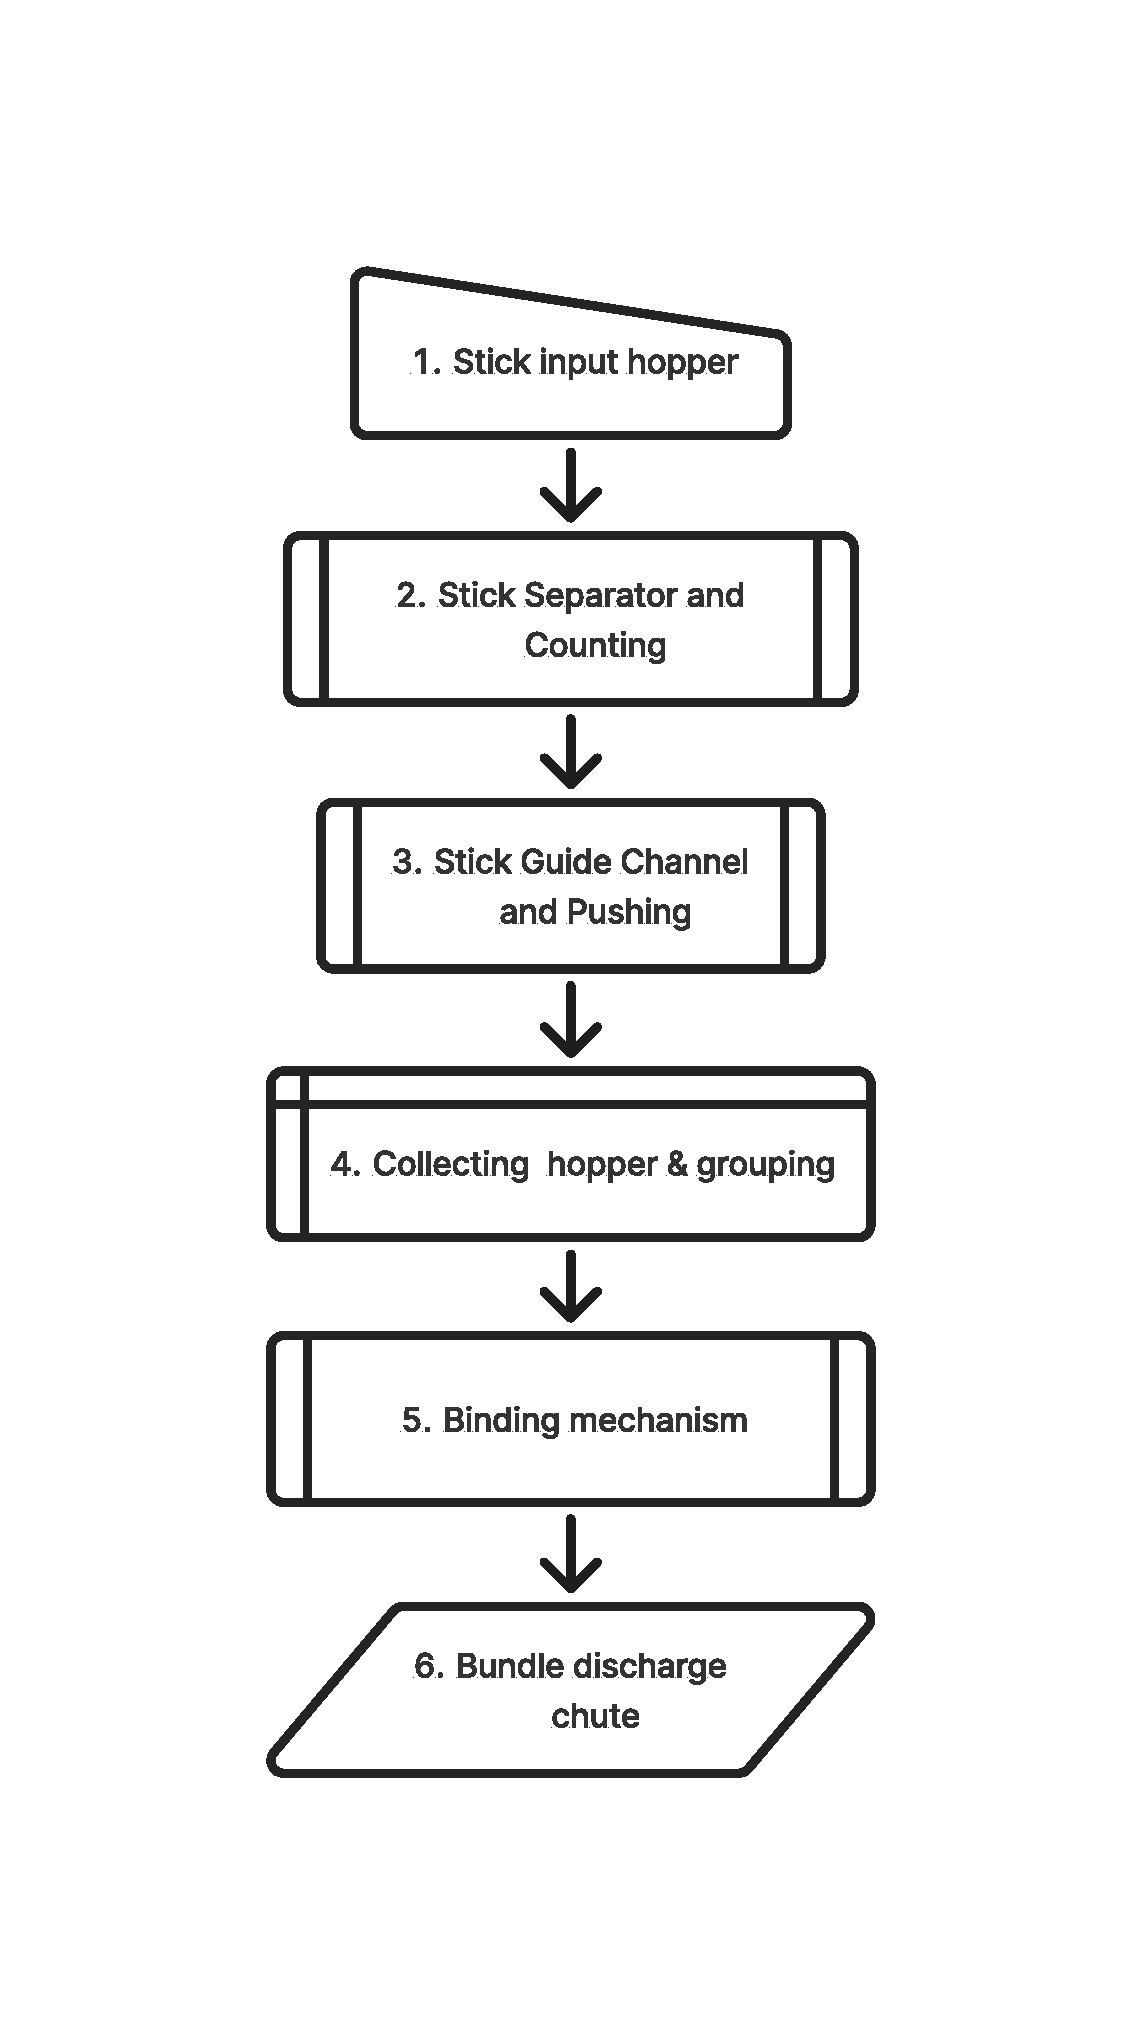
\includegraphics[
%   width=\textwidth,
%   height=0.5\textheight,
%   keepaspectratio
% ]{images/functional-flow.pdf}
% \caption{Functional block diagram of the mechanical counting and bundling machine.}
% \label{fig:functional-flow}
% \end{figure}

\section{Overall Design and Analysis Workflow}

Design and analysis will begin with concept generation and selection, followed by detailed kinematic design of the indexing mechanism. CAD modeling will be used to refine the design, followed by kinematic and dynamic analysis and finally testing and documentation. 

Iterative adjustments will be made based on test results to optimize performance and reliability. Flow charts (Fig. \ref{fig:design-analysis}) will be used to validate the sequence of operations and identify potential failure points for mitigation.

\begin{figure}[!htbp]
    \centering
    % Left Figure
    \begin{subfigure}[b]{0.46\textwidth}
        \centering
        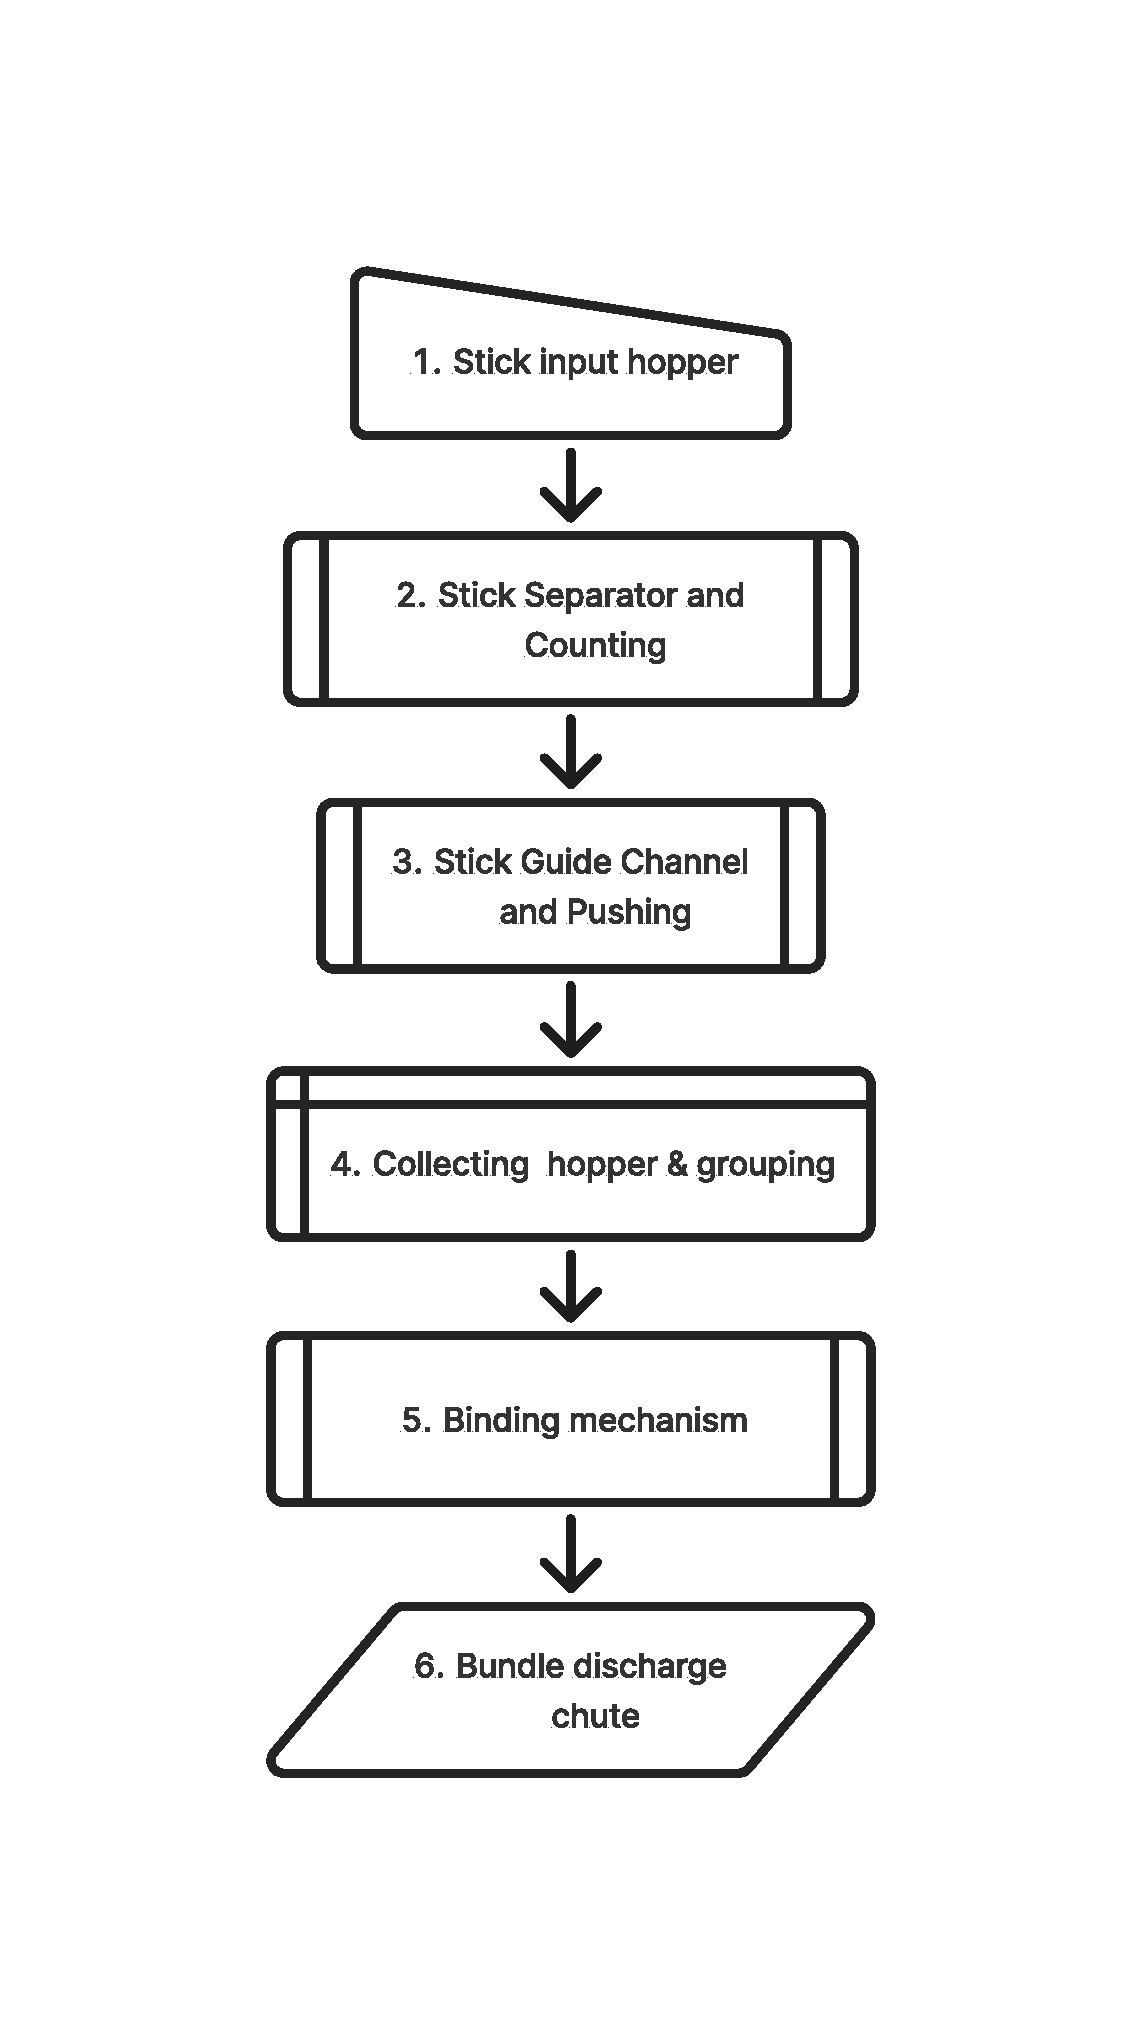
\includegraphics[width=\textwidth, height=0.8\textheight, keepaspectratio]{images/functional-flow.pdf}
        \caption{Functional block diagram of the mechanical counting and bundling machine.}
        \label{fig:functional-flow}
    \end{subfigure}
    \hfill % Adds horizontal space between the two figures
    % Right Figure
    \begin{subfigure}[b]{0.46\textwidth}
        \centering
        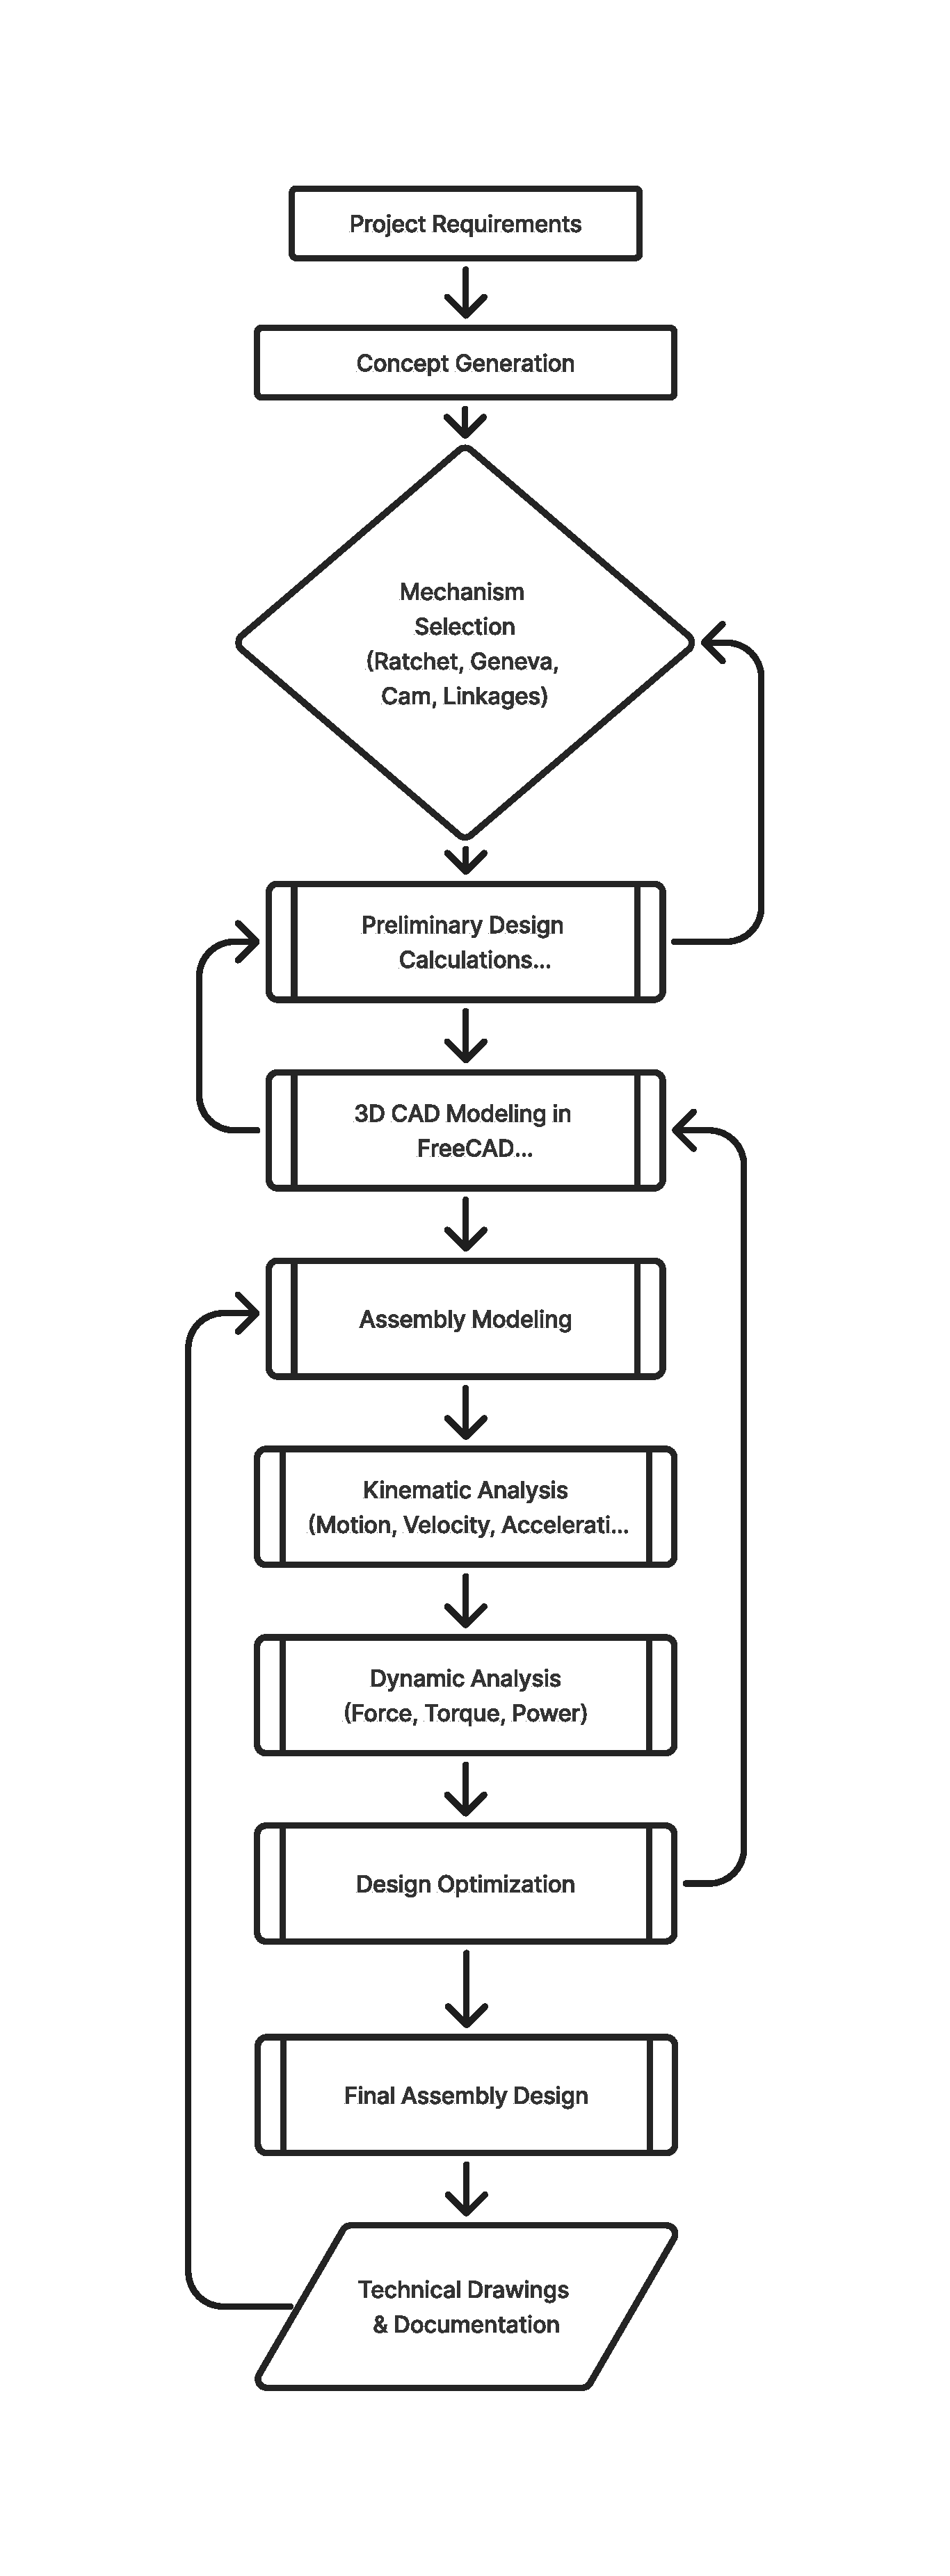
\includegraphics[width=\textwidth, height=0.8\textheight, keepaspectratio]{images/design-analysis.pdf}
        \caption{Flow chart depicting the sequence of operations and decision points for the mechanical counting and bundling machine.}
        \label{fig:design-analysis}
    \end{subfigure}
    
    % Optional: Overall main caption for both figures combined
    \caption{System block diagram and process flowchart.}
\end{figure}


\section{CAD Modeling and Simulation}
CAD software (SolidWorks) will be used for 3D modeling of the mechanism, allowing for detailed design and interference checks. Kinematic analysis will be performed to ensure the desired motion profiles are achieved, while dynamic analysis will evaluate forces and stresses to inform material selection and structural design. Simulation results will be validated against theoretical calculations to ensure accuracy and reliability of the design before prototyping. Flow chart \ref{fig:cad-wrokflow} shows a typcial .

\begin{figure}[!htbp]
	\centering
	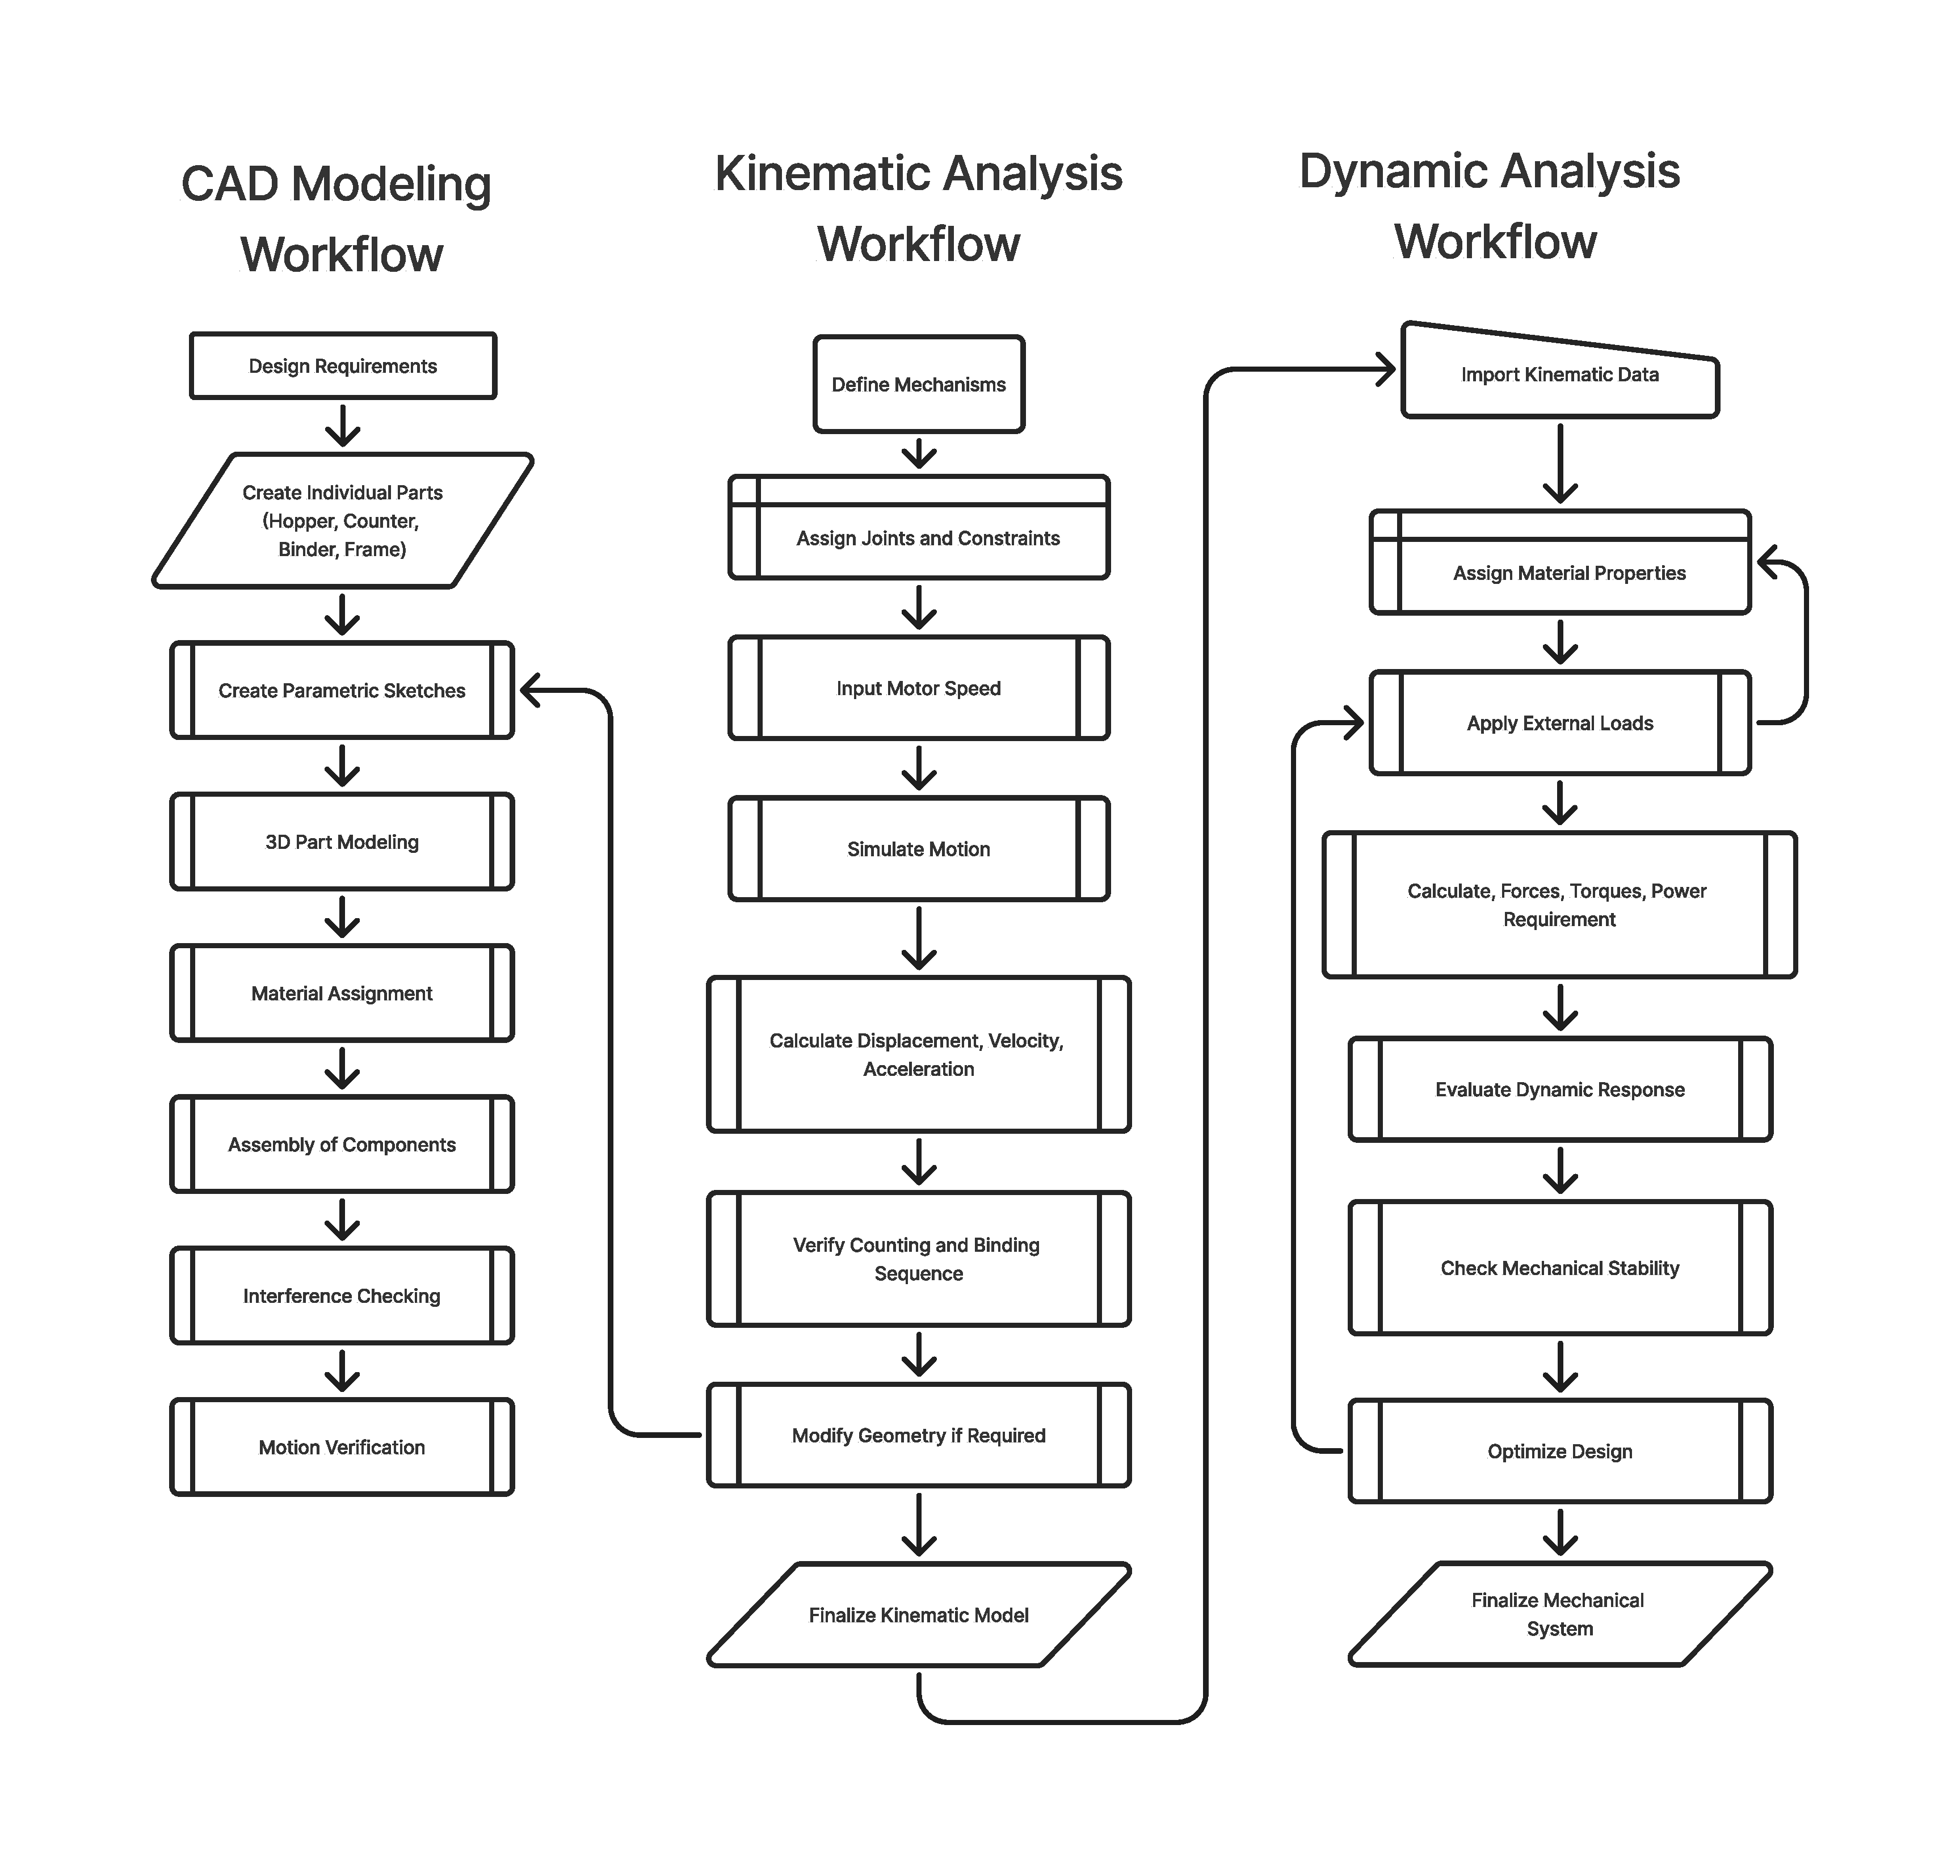
\includegraphics[width=\textwidth, height=0.8\textheight, keepaspectratio]{images/cad-workflow.pdf}
	\caption{Flow chart illustrating the CAD modeling and simulation workflow for the mechanical counting and bundling machine.}
	\label{fig:cad-wrokflow}
\end{figure}


\chapter{Result And Analysis}
\label{result}
\section{Expected Output}
The prototype is expected to deliver grouped sets of incense sticks at a predictable count per cycle with low variance. Initial throughput targets are 30-120 groups per minute depending on drive method and operator skill.

% \figure[htbp]
% \centering
% \includegraphics[width=0.8\textwidth]{images/prototype.jpg}
% \caption{Preliminary prototype design for mechanical counting and bundling of incense sticks.}
% \label{fig:prototype}

\section{Performance Metrics}
Key metrics to evaluate the design include:
\begin{itemize}
	\item Counting accuracy (items per group vs target)
	\item Throughput (groups per minute)
	\item Mean time between jams (MTBJ)
	\item Wear indicators (visual inspection of guides, pins)
	\item Energy input per cycle (if motorized)
\end{itemize}

\section{Success Criteria}
The design will be considered successful if it achieves $\geq 95\%$ counting accuracy, meets a practical throughput for small-scale production, and can be fabricated and maintained at a low cost.

\section{Future Work}
Future improvements may include simplifying the binding mechanism, adding lightweight sensing for automated reject handling, and optimizing cam profiles for smoother operation.

\chapter*{Gantt Chart}
\addcontentsline{toc}{chapter}{Gantt Chart}
\label{ganttchart}
\clearpage
\begin{landscape}
\thispagestyle{plain}
\begin{center}
\vspace*{\fill}
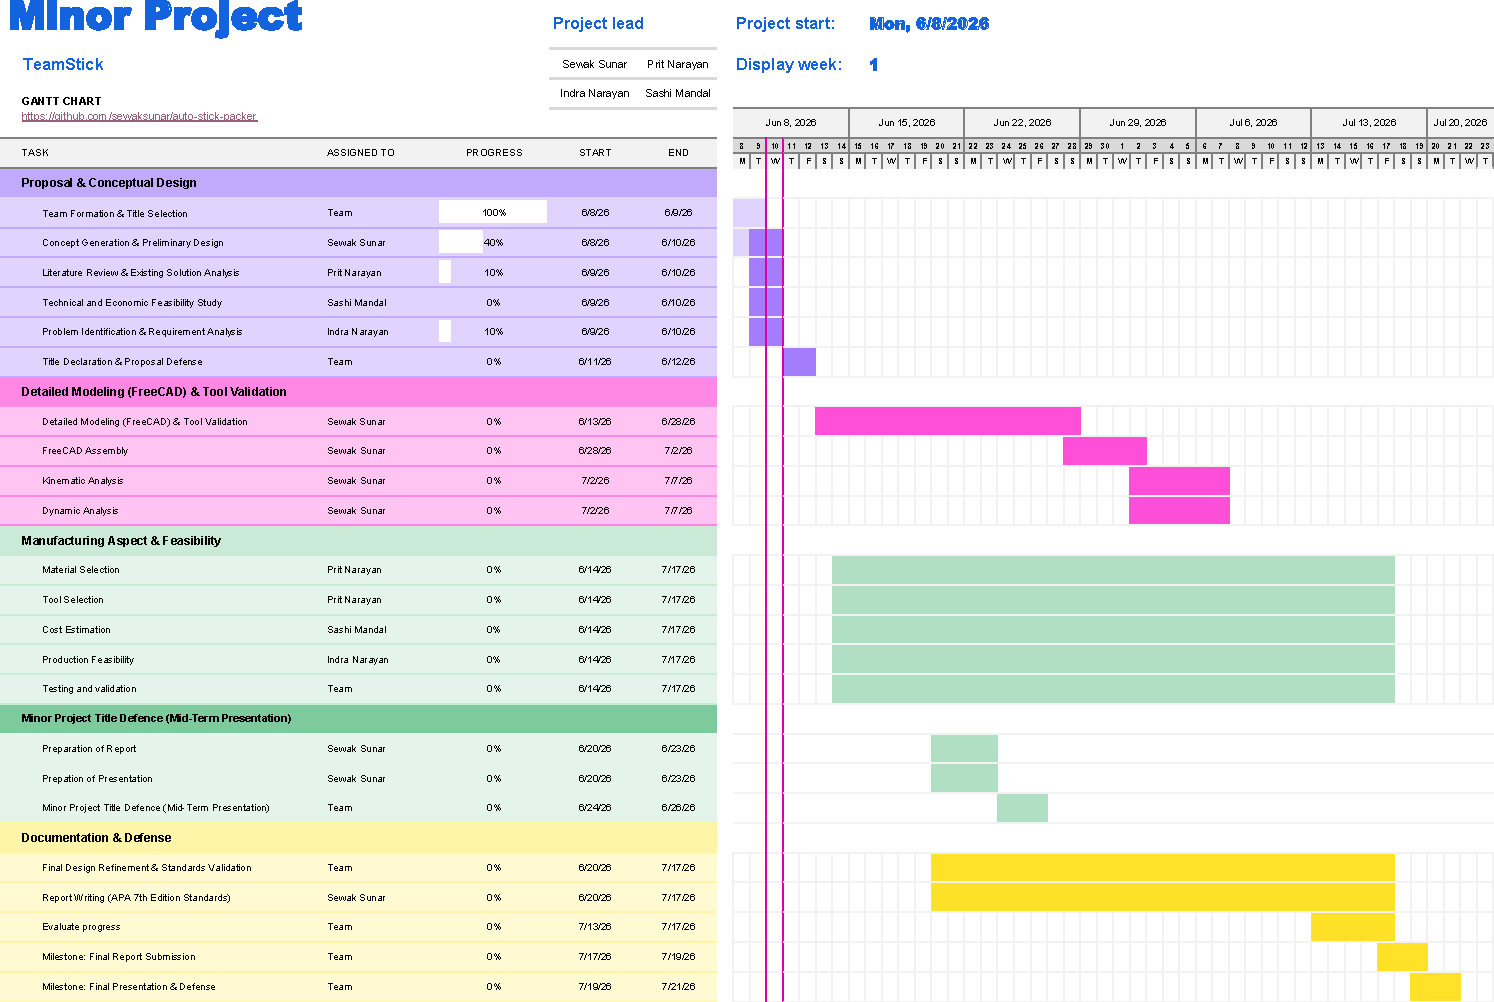
\includegraphics[
    width=2\linewidth,
    height=0.9\textheight,
    keepaspectratio
]{images/gantt-chart.pdf}
\vspace{1em}
% \captionof{figure}{Gantt chart illustrating the project timeline and key milestones for the design and analysis of the stick counting and packaging system.}
\label{fig:gantt-chart}
\vspace*{\fill}
\end{center}
\end{landscape}
\clearpage


\chapter*{References}
\addcontentsline{toc}{chapter}{References}
\label{references}
% Use thebibliography's heading and add it to the TOC without duplicating
\phantomsection
\addcontentsline{toc}{chapter}{References}
\begin{thebibliography}{9}

\bibitem{shigley2011}
J. E. Shigley and C. R. Mischke,
\textit{Mechanical Engineering Design}, 9th ed., McGraw-Hill, 2011.

\bibitem{norton2011}
R. L. Norton,
\textit{Machine Design: An Integrated Approach}, 4th ed., Prentice Hall, 2011.

\bibitem{juvinall2003}
R. C. Juvinall and K. M. Marshek,
\textit{Fundamentals of Machine Component Design}, 4th ed., Wiley, 2003.

\bibitem{lit1}
Representative articles and manufacturer datasheets on cams, Geneva mechanisms, and small drive motors were consulted during design; these are cited in the final report where specific values are used.

\end{thebibliography}

\end{document}
